\chapter{Capitulo Auxiliar}

Toda documentação pode ser encontrada aqui. \url{https://www.overleaf.com/learn/latex/Main_Page}

IMPORTANTE, para quebrar a linha, como um novo paragrafo, deve ter uma linha em branco.

COM LINHA EM BRANCO

Nome do capítulo

Nivel X.
SEM LINHA EM BRANCO 
Nome do capítulo
Nivel X.

\section{Nome do Subcapitulo}

Exemplo 3.1 Objetivos gerais

Nivel X.Y

\subsection{Nome Item}
Nivel X.Y.X


\subsubsection{Nome do SubItem}

Nível X.Y.Z.A

\paragraph{Nome do paragráfo}

Nivel X.Y.Z.A.B


\section{Usando Equações}

Latex possui uma linguagem específica para incluir equações. Muito prática e fácil quando se conhece os códigos. Para facilitar quando não se conhece é possível usar o site

\url{https://www.codecogs.com/latex/eqneditor.php?lang=pt-br}

E ir montando cada equação nele. E então substituir no bloco abaixo. As legendas das equações podem ser incluídas no bloco conditions. 

\begin{equation}\label{eq:freq_per}
    f=\frac{1}{T} % colar a nova equação aqui
\end{equation}%

\begin{conditions*}
 f  &  Frequência de oscilação (Hz)\\
 T  &  Período de oscilação (s)
\end{conditions*}


\section{Usando imagens}

Para a adição de imagens no documento é necessário salvas antes no projeto. Por isso é importante salvar sempre na pasta img, e com um nome fácil de se identificar.

\begin{figure} [H]
    \vspace{1.0em}
    \centering%
    \caption{Graus de liberdade de um sistema}% Título da imagem
    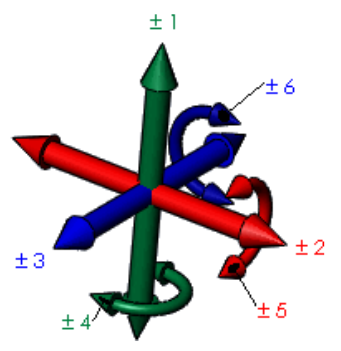
\includegraphics[width=.25\textwidth]{../img/graus_liberdade_solidworks.png}% Nome da imagem com a extensão, ex: .png, .jpg aqui
    \\\hspace{\linewidth}%
    \textbf{Fonte:} \cite{solidWorks} % Fonte da imagem
    \label{fig:graus_liberdade} 
    \vspace{1.0em}
\end{figure}

Para adicionar um figura com duas imagens, temos que utilizar o bloco subfloat. para cada imagem. Como visto abaixo. e 
 
\begin{figure}[H]
    \vspace{1.0em}
    \centering
    \caption{Oscilação do Pendulo no plano Tempo x Amplitude}
    \subfloat[Movimento do Pendulo]{ % titulo da subimagem
        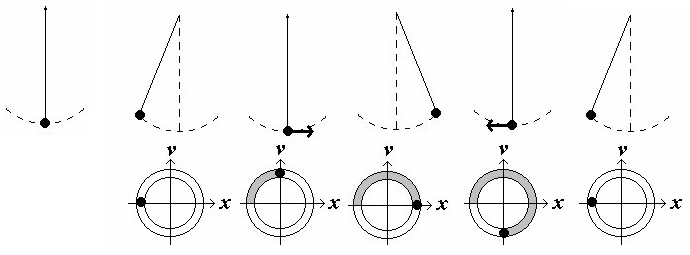
\includegraphics[width=.6\textwidth]{../img/movimento_pendulo_wiki.png}%
        \label{fig:pendulo_movimento}
    }
    \subfloat[Movimento circular no plano]{
        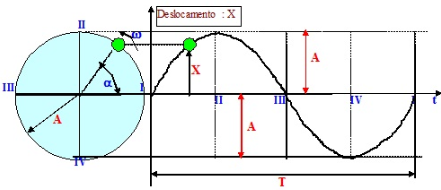
\includegraphics[width=.4\textwidth]{../img/grafico_fta_propria.png}%
        \label{fig:grafico_fta}
    }
    \hspace{\linewidth}%
    \textbf{Fonte:} do Autor%
    \label{fig:cefets}
    \vspace{1.0em}
\end{figure}


O próprio Latex ja organiza as imagens com o tamanho da folha, então para inclui duas linhas é so incluir mais subfloats.

\begin{figure}[H]
    \vspace{1.0em}
    \centering
    \caption{Forças de excitação}
    \subfloat[Força harmônica]{
        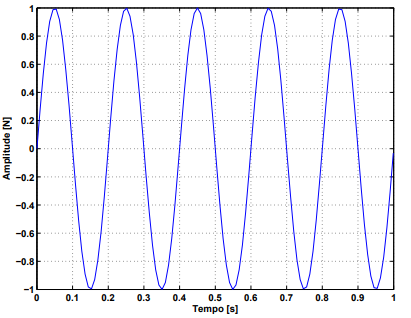
\includegraphics[width=.45\textwidth]{../img/forca_harmonica_daSilva.png}%
        \label{fig:forca_excitacao_harmonica}
    }
    \subfloat[Força periódica]{
        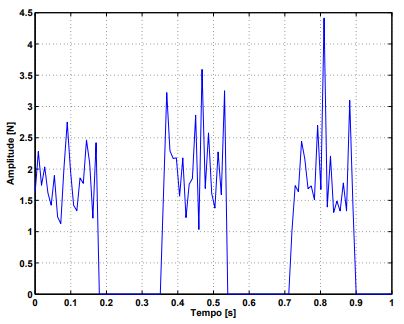
\includegraphics[width=.45\textwidth]{../img/forca_periodica_daSilva.png}%
        \label{fig:forca_excitacao_periodica}
    }
    
    \subfloat[Força transitória]{
        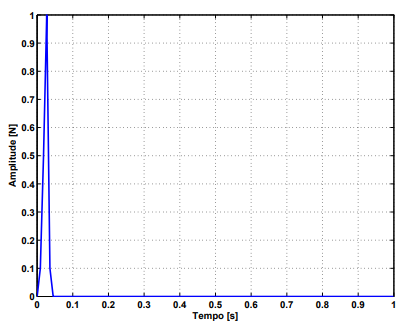
\includegraphics[width=.45\textwidth]{../img/forca_transitoria_daSilva.png}%
        \label{fig:forca_excitacao_transitoria}
    }
    \subfloat[Força aleatória]{
        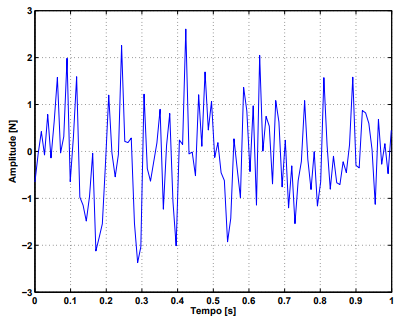
\includegraphics[width=.45\textwidth]{../img/forca_aleatoria_daSilva.png}%
        \label{fig:forca_excitacao_aleatoria}
    }
    \hspace{\linewidth}%
    \textbf{Fonte:} \cite{daSilva}%
    \label{fig:forca_excitacao}
    \vspace{1.0em}
\end{figure}


\section{Usando tabelas}

Editar tabelas no latex não é tão prático. Mas aqui tem um site que ajuda na conversão da tabela de excel para o formato latex. \url{https://www.tablesgenerator.com/}

Depois é so editar seguindo o template abaixo.


    \begin{table}[H]
        \vspace{1.0em}
        \centering%
        \caption{Cronograma previsto para continuidade do trabalho}%
        \begin{tabular}{p{9cm}p{3cm}p{3cm}}% Aqui é possível definir o tamanho de cada coluna. 
            \hline
            \textbf{Atividade prevista}  & \textbf{Início prevista} & \textbf{Final prevista}\\
            \hline
            Estudo dos dados experimentais                      &   Fevereiro/2020   &   Fevereiro/2020 \\
            Criação do modelo computacional                     &   Fevereiro/2020   &   Março/2020 \\
            Teste com novos valores e propostas de melhoria     &   Março/2020       &   Abril/2020 \\
            Ajuste final do modelo para resolução do problema   &   Abril/2020       &   Maio/2020 \\
            Teste final do modelo computacional                 &   Abril/2020       &   Junho/2020 \\
            Compilação dos resultados                           &   Maio/2020        &   Junho/2020 \\
            Finalização do relatório escrito                    &   Maio/2020        &   Junho/2020 \\
            Apresentação do trabalho                            &   Julho/2020       &   Julho/2020 \\
            \hline
        \end{tabular}
        \\\hspace{\linewidth}%
        \textbf{Fonte:} Autoria do Autor%
        \label{table:cronograma}
        \vspace{1.0em}
    \end{table}

\section{Usando citações}

As citações podem ser divididas em duas partes. 

\subsection{Criando referências}
Antes de indicar um elemento precisamos cria-lo.

\subsubsection{Para imagens, tabelas e equações}
Para estes elementos incluimos a tag \ label para criar essa referência. Assim é primeiro definido o tipo do elemento (table, eq, fig) e o nome para usar na referência.

\subsubsection{Para símbolos/constantes}
É o caso de letras gregas, e símbolos diversos. Eles precisam ser criados no aquivo simbolos.tex dentro da pasta lista. Seguindo o modelo comentado abaixo.
% \nomenclature{$C_c$}{Amortecimento crítico  (Ns/m ou kg/s)}

\subsubsection{Para Glossário}
Estes devem ser criados na primeira parte do arquivo glossario.tex dentro da parte listas. Seguindo o modelo comentado abaixo

%\newglossaryentry{output}{   
%    name=output,
%    description={Informação ou dado que é utilizado como dado de saída para um problema}
%}

\subsubsection{Para abreviações}
Eles precisam ser criados no aquivo abreviacoes.tex dentro da pasta lista. Seguindo o modelo comentado abaixo. 

O primeiro argumento é o nome da referência, o segundo a abreviação, e o terceiro a definição.
%\newacronym{nvh}{NVH}{Noise, Vibration and Harshness}

\subsubsection{Para referências bibliográficas}

Estas precisam ser incluídas com bastante atenção. Inicialmente acesse o aquivo refs.bib. Nele é possível ver diversos tipos de referências, seja artigo (article), livro(book), mic(notas de aula), online(sites), entre outros. Estas definições são necessárias para a organização das referências no final do documento.

Seguindo para sua definição, o primeiro argumento indica o nome da referência, e os outros tem o seu tipo definido. Vejo no texto comentado abaixo

%@book{rao,
%    title = {Mechanical Vibrations},
%    author = {Singiresu S. Rao},
%    isbn= {978-0-13-212819-3},
%    year = {2011},
%    publisher = {Prentice Hall},
%    keywords = {vibration}
%}

\subsection{Citando as referências}
Existem diversas formas para referenciar algo.


\subsubsection{Para imagens, tabelas e equações}
Devemos usar a tag \ ref incluindo o tipo e nome da imagem, tabela ou equação. Como aqui: \ref{fig:forca_excitacao_harmonica}

\subsubsection{Para símbolos/constantes}
Símbolos/Constantes podem ser referenciados como no exemplo ao lado, indicando o nome criado no arquivo simbolos.tex: \(m\)

Isso não consiste numa referência propriamente, mas deixa o texto em itálico, e é o suficiente para poder dar destaque à constante.

\subsubsection{Para glossário}
Existem várias formas para referência um termo do glossário, e são usados variações para \ gls. Como visto nos comentários abaixo

%\gls{ } imprimir em caixa baixa
%\Gls{ } imprimir com a primeira letra em caixa alta


\subsubsection{Para abreviações}
Existem várias formas para citar uma abreviação, podendo ser apenas a sigla, a definição, ou a definição seguida pela sigla entre parênteses. Como visto no comentário abaixo:

%\newacronym{cefetmg}{CEFET-MG}{Centro Federal de Educação Tecnológica de Minas Gerais}
%\acrlong{ }  \acrlong{cefetmg} exibe Centro Federal de Educação Tecnológica de Minas Gerais.
%\acrshort{ } \acrshort{cefetmg} exibe CEFET-MG
%\acrfull{ }  \acrfull{cefetmg} exisbe Centro Federal de Educação Tecnológica de Minas Gerais (CEFET-MG)


\subsubsection{Para referências bibliográficas}
Para citar referências bibliográficas podemos utilizar diversas formas, podendo pegar apenas o autor, ou o titulo do trabalho, e etc. As duas primeiras podem ser utilizadas no TTC.

\cite{rao}

\parencite{rao}

\citeauthor{rao}

\citetitle{rao}

\section{Alguns materiais de consulta}


\url{http://each.uspnet.usp.br/sarajane/wp-content/uploads/2016/10/manual-latex-1.pdf}

\url{http://tug.ctan.org/info/biblatex-cheatsheet/biblatex-cheatsheet.pdf}

\section{Informações úteis}


O compilador usado é o XeLatex. Caso tenho erro ao visualizar o documento, confira esta configuração no botão menu a esquerda.

Duas teclas \ \ forçam o compilador pular para a linha de baixo

Se uma referência é criada, mas não usada ela não é exibida na lista de imagem/tabelas, glossário, ou abreviações. O mesmo não vale para a lista de constantes.

Clicar duas vezes num texto no lado do PDF, direciona o lado do Latex para a mesma região.